\chapter{Classification networks}
\label{sec:clsnets}
A fundamental building block for a modern state-of-the-art image classification network is a convolutional layer. Accordingly, we call this type of networks a convolutional neural networks (CNN) \cite[ch.~9]{bib:dlbook}. CNN based classifier is a network that given the input image, extracts a feature map from this image and then applies classification layers to produce a confidence score for each possible class. Usually, the soft-max function is applied to the confidence score to get a probability distribution.

We use this section to take a walk through the history of classification CNNs and outline some of the most influential models. Some of those models are still used, and others are responsible for inspiring the next generations of even better networks.

\section{AlexNet (2012)}
AlexNet designed by \citeauthor{bib:alexnet} \cite{bib:alexnet} is the first CNN that won the ILSVRC challenge over traditional computer vision and machine learning approaches. It created a foundation on which today's state-of-the-art models are built, and set a new standard for image recognition. AlexNet is created from a stack of five convolutional layers interleaved by max-pooling layers, followed by two fully connected layers and a softmax layer. It also popularized the use of ReLU non-linearity in CNNs.

\section{VGG (2014)}
\label{sec:VGG}
The network architecture, mostly known as VGG, by \citeauthor{bib:vgg} \cite{bib:vgg}, is built on the deep CNN concept behind AlexNet. It managed to prove the feasibility of even deeper network utilizing small convolution filters. 

Each of the VGG's convolutional filters employs a 3$\times$3 kernel with the depth of the feature map gradually increasing through the network. The convolutions are followed by three fully connected layers and softmax layer, see \cref{tab:vggarch}. 

Multiple versions of the VGG architecture can be constructed, depending on the number of convolutional layers. The most popular is the 16 layer version, titled VGG-16.

Today the VGG network is considered to be a general architecture for a classification network due to its linear architecture with a decreasing area of the features, and an increasing number of channels. 

\begin{figure}
    \centering
    \rotatebox{90}{
        \vggArch
    }
    \caption[VGG-16 architecture]%
    {Architecture of VGG network version D, commonly called VGG-16. Other versions in \cite[table 1]{bib:vgg}.}
    \label{tab:vggarch}
\end{figure}

\section{Inception (2014)}
\label{sec:inception}
Predating architectures suggest that increasing the number of layers and layer size, leads to better precision. \citeauthor{bib:googlenet} introduced Inception v1 \cite{bib:googlenet}, also known as \textit{GoogLeNet}, with the goal of increasing precision while improving utilization of computing resources.

Although stacking more convolutional layers improves the accuracy, an increasing computational cost of those layers quickly overpowers the benefits. To avoid the aforementioned cost, Inception introduces the concept of sparsity in convolutional layers. The sparsity is achieved by using \textit{inception modules} that approximate a sparse structure by utilizing multiple convolutions with different kernel sizes and concatenating the outputs together (see \cref{fig:incept_mod}). 

To reduce the computational cost further, each convolution is preceded with additional 1$\times$1 convolution, used for a dimensionality reduction. An alternate path in the \textit{inception module} is provided by max-pooling operation and concatenating it to the output.

Inception begins with a sequence of convolution, pooling, and local response normalization operations. This 'stem' is followed by a chain of nine \textit{inception modules}, topped by a fully connected soft-max classifier. Two auxiliary classifiers are added to intermediate layers of the network to help propagate gradients and provide regularization during the training.

\subsection*{Inception v2, v3 (2015)}
A set of improvements to the Inception network is introduced in later versions of the network. Most notably a factorization of convolution layers in Inception v2 and v3, \citeauthor{bib:inception2} \cite{bib:inception2}. Factorization replaces larger convolutions with a network of many smaller ones. They found this method very effective, e.g., replacing a 5$\times$5 convolution with two layers of 3$\times$3 results in a relative gain of 28\% and replacing 3$\times$3 layer with 3$\times$1 and subsequent 1$\times$3 layer is 33\% cheaper.

\begin{figure}
    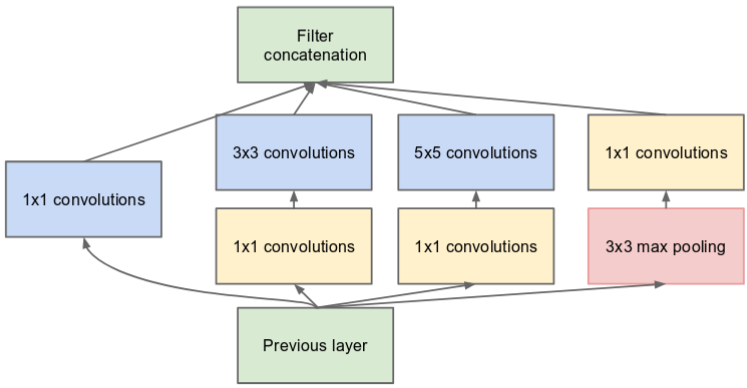
\includegraphics[width=\textwidth]{img/inception}
    \caption[Inception module]%
    {Inception module, picture from \cite[figure 2]{bib:googlenet}.}
    \label{fig:incept_mod}
\end{figure}

\section{ResNet (2015)}
\label{sec:resnet}
A trend of adding more layers to CNNs to achieve better accuracy has pushed the limit towards networks with hundred or more layers.  Theoretically, adding more layers to a model should produce equal or better results, based on the fact that shallow model is the subspace of the deeper one. Therefore, additional layers can learn to forward the data. In practice, however, observations suggest that this is not the case, and very deep networks can experience eventual degradation. A solution to this problem was proposed by \citeauthor{bib:resnet} \cite{bib:resnet} in the ResNet architecture by directly introducing identity functions to the network.

Basic principles of ResNet are directly inspired by the VGG. Most of the convolutional layers use 3$\times$3 filters and follow two simple rules: keep the number of filters the same, unless changing the output size and double the filters if the feature size if halved. A newly introduced residual connection bypasses each pair of the convolutional layers and forms a \textit{residual blocks}. This connection can be an identity function or a 1$\times$1 convolution to match the increased number of filters.

\begin{figure}
    \resnetArch
    \caption[ResNet architecture]%
    {Architecture of the ResNet network and residual blocks. Each of the four \textit{Layers} is created by stacking multiple residual blocks.}
    \label{fig:resnet_arch}
\end{figure}

We can see the high level architecture of this model in \cref{fig:resnet_arch} (left). Each of four \textit{Layers} represents a sequence of multiple residual blocks, exact numbers of blocks can be found in \cite[table 1]{bib:resnet}. Previously described \textit{residual block} with two convolutional layers, known as \textit{Basic block}, is used for smaller ResNet models (ResNet18, ResNet34). Deeper ResNet models (ResNet50, ResNet101, ResNet152) use the \textit{Bottleneck block} with three convolutional layers. In \textit{Bottleneck block}, the 1$\times$1 layers are responsible for reducing and then restoring dimensions, allowing for faster 3$\times$3 layer with reduced input and output dimensions. Thanks to the efficient architecture, the 152-layer ResNet has lower computational complexity than the 16-layer VGG network.



\section{Xception (2017)}
\label{sec:xception} Xception architecture by \citeauthor{bib:xception} \cite{bib:xception}, is heavily inspired by previous architectures, mainly Inception and ResNet. It is built on the hypothesis claiming: "the mapping of cross-channel correlations and spatial correlations in the feature maps of convolutional neural networks can be entirely decoupled." This hypothesis expands upon the hypothesis underlying Inception architectures. Therefore the name 'Extreme Inception.' 

The hypothesis is realized in the form of \textit{depthwise separable convolution} layers (shortly separable convolution). Depthwise separable convolution consists of two steps: a \textit{depthwise convolution} and \textit{pointwise convolution}. A depthwise convolution is a convolution performed independently over each channel, i.e., a convolution without changing the number of channels. The second step is a pointwise convolution that uses 1$\times$1 kernel to map the output of depthwise convolution into new channel space.

The model is formed by linearly stacking separable convolution layers with the addition of residual connections as seen on \cref{fig:xception}. Convolutional layers, non-linearity, and poolings are structured into residual blocks similarly to ResNet architecture.

\begin{figure}
    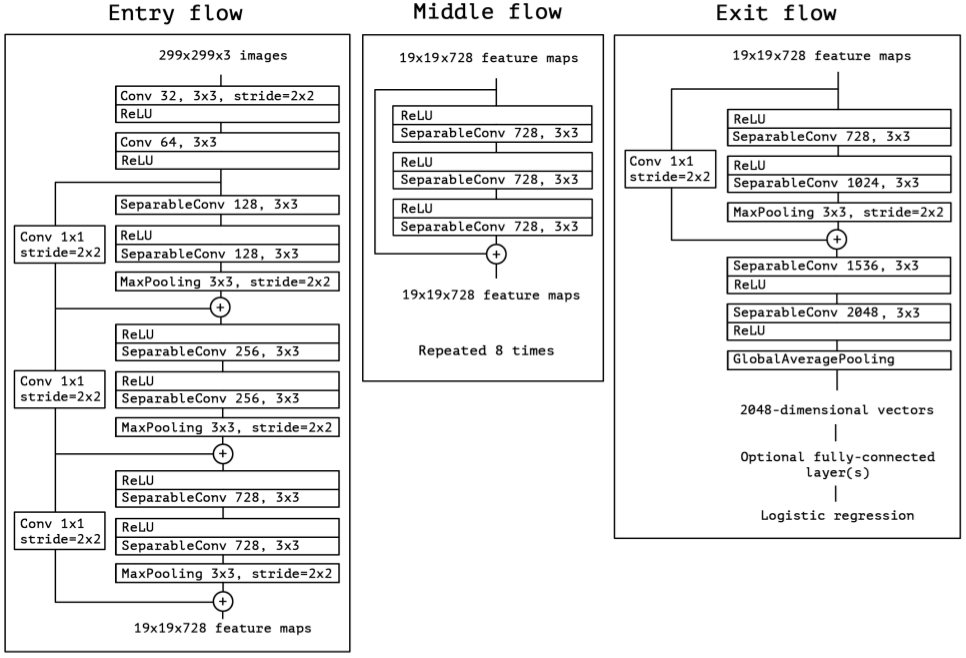
\includegraphics[width=\textwidth]{img/xception}
    \caption[Xception architecture]%
    {Structure of \textit{Xception} architecture. Taken from \cite[fig. 5]{bib:xception}.}
    \label{fig:xception}
\end{figure}


\section{NASNet (2017)}
\label{sec:nasnet}
This architecture stands out from others mentioned because \citeauthor{bib:nasnet} \cite{bib:nasnet} used a machine learning algorithm to design the network. It is a result of a \textit{AutoML}\footnote{\url{https://ai.googleblog.com/2017/05/using-machine-learning-to-explore.html}} project. Unlike manually designing the network by trial and error, AutoML searches the space of all possible models, e.g., using reinforcement learning and evolutionary algorithms. This approach is limited by the computational cost and therefore limited to small datasets.

NASNet is a result of taking an architecture designed for small \textit{CIFAR-10}\footnote{\url{https://www.cs.toronto.edu/~kriz/cifar.html}} dataset by AutoML and using it to create larger model for ImageNet dataset. The model is composed of two types of learned cells, a \textit{Normal Cell} and \textit{Reduction Cell} (see \cref{fig:nasnet}). A general structure of the network is then created by alternating a Reduction Cell and \textit{N} Normal Cells.

\begin{figure}
    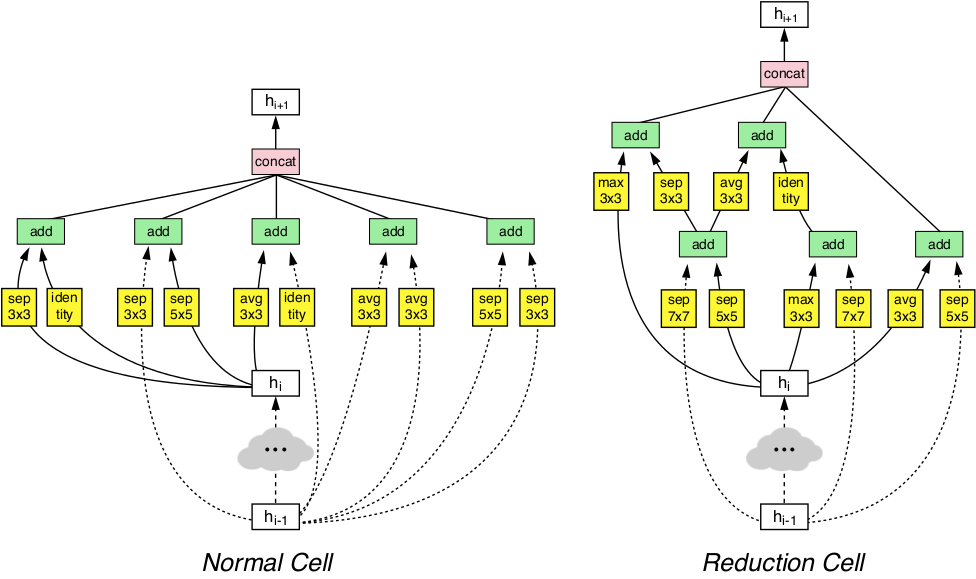
\includegraphics[width=\textwidth]{img/nasnet}
    \caption[NASNet-A modules]
    {Modules used in \textit{NASNet-A}, designed by AutoML. Image from \url{ai.googleblog.com/2017/11/automl-for-large-scale-image}.}
    \label{fig:nasnet}
\end{figure}

\section{Comparing the classifiers}
\label{sec:cnncomp}
At the beginning of this chapter, we mentioned that the classification networks are often compared based on performance on the ImageNet dataset. Newer models, like Xception, NASNet, and modifications of ResNet reach excellent accuracy. However, there is a large discrepancy in their performance considering inference speed. In \cref{fig:cnnbenchmark} we provide an overview of fps--accuracy relationship taken from an independent benchmark by \citeauthor{bib:cnnbenchmark} \cite{bib:cnnbenchmark}. Although the experiment was performed with batch size 1, we expect a universal increase of fps with a bigger batch and only small changes to the relative performance of different models. We can observe a clear trade-off between speed and accuracy for the classification task.

\begin{figure}
    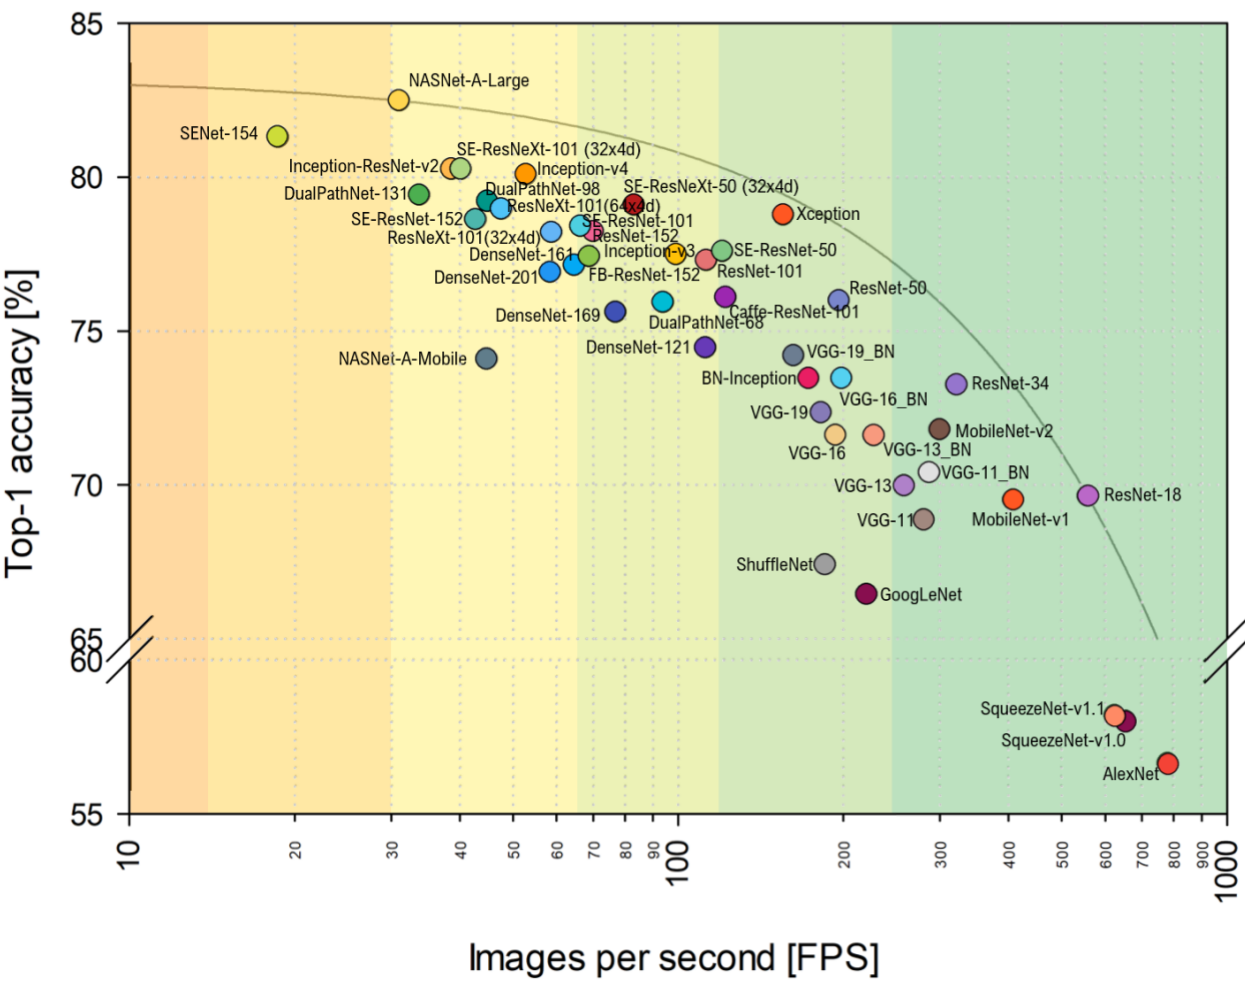
\includegraphics[width=\textwidth]{img/fps_comp}
    \caption[Benchmark of classification CNNs]%
    {Benchmark of state-of-the-art classification deep neural networks on \textit{ILSVRC} dataset. Performed on NVIDIA
Titan X GPU with batch size 1. Taken from \cite[fig. 3]{bib:cnnbenchmark}}
    \label{fig:cnnbenchmark}
\end{figure}
